%!TEX root = main.tex


Let us begin by reviewing the concept of \emph{constrained optimization}, and some associated notation and terminology.  The objective is the search for extrema of a function $f \colon D \to \field{R}$ where the input values $\x$ belong in an open subset $D \subseteq \field{R}^d$ and satisfy a finite set of \emph{constraints} of the form
\begin{gather*}
g_1(\x) \leq 0, g_2(\x) \leq 0, \dotsc, g_m(\x) \leq 0, \\
h_1(\x) = 0, h_2(\x) = 0, \dotsc, h_\ell(\x) = 0,
\end{gather*}
for real-valued functions $g_k\colon \field{R}^d \to \field{R}, (1\leq k \leq m)$, $h_k \colon \field{R}^d \to \field{R}, (1\leq k \leq \ell)$.
\index{Constrained optimization}
\index{Constraint}

For simplicity, we write instead
\begin{equation}\label{equation:programP}
(P) \begin{cases} \min_{x\in D}f(\x) \\ g_1(\x) \leq 0, \dotsc, g_m(\x) \leq 0 \\ h_1(\x) = 0, \dotsc, h_\ell(\x) =0 \end{cases}
\end{equation}
or better, if we set 
\begin{equation*}
S = \{ \x \in D : g_1(\x) \leq 0, \dotsc, g_m(\x) \leq 0, h_1(\x) = 0, \dotsc, h_\ell(\x)=0\},
\end{equation*} we may simply write 
\begin{equation*}
(P) = \min_{x\in S} f.
\end{equation*}
We refer to it as the \emph{program} $(P)$.\index{Program} The function $f$ is called the \emph{objective function of }$(P)$\index{Objective function of $(P)$}.  We refer to the functions $g_k$ as the \emph{inequality constraints}.  The functions $h_k$ are called the \emph{equality constraints}.\index{Constraint!inequality}\index{Constraint!equality}

A point $\x \in D$ that satisfies all the constraints of the program $(P)$ is said to be \emph{feasible}.\index{Feasible!point}  The set of all feasible points is called the \emph{feasibility region} of $(P)$.\index{Feasibility region}  If the feasibility region is non-empty, we say that the program $(P)$ is \emph{consistent}\index{Program!consistent}. If a feasible point satisfies $g_k(\x) < 0$ for all inequality constraints, we call it a \emph{Slater point}\index{Slater point}. Consistent programs $(P)$ that have Slater points are said to be \emph{super-consistent}.
\index{Program!super-consistent}

If the objective function $f$ and all constraints $g_k$, $h_k$ of a program $(P)$ are linear functions, we denote it by $(LP)$ and refer to it as a \emph{linear program}.  If the objective function, all constraints $g_k$, $h_k$ and the set $D$ are convex, we call $(P)$ a \emph{convex program}.
\index{Program!linear}\index{Program!convex}

\begin{example}\label{example:feasibleP1}
Let $f(x,y)=x^4+y^4$, and consider the program $(P) = \min_{x\in S} f(x,y)$, where $S = \{ (x,y) \in \field{R}^2: x^2 \leq 1, y^2 \leq 1, e^{x+y}\leq 1\}$.

The inequality constraints are $g_1(x,y)=x^2-1$, $g_2(x,y)=y^2-1$ and $g_3(x,y)=e^{x+y}-1\leq 0$ (although you may choose simpler equivalent expressions).  The feasibility region is thus a triangular region (see Figure \ref{figure:feasibleP1}):
\begin{equation*}
S = \{ (x,y) \in \field{R}^2 : \abs{x} \leq 1, \abs{y} \leq 1, x+y \leq 0 \} \neq \emptyset.
\end{equation*}
\begin{figure}[ht!]
\begin{tabular}{cc}
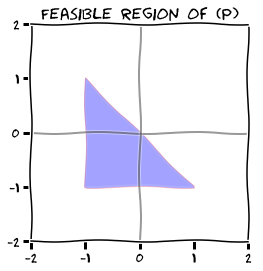
\includegraphics[width=0.5\linewidth]{images/feasibleP1.png} &
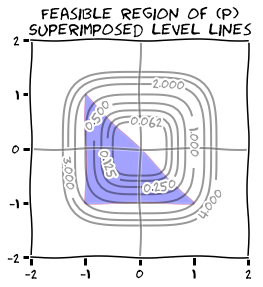
\includegraphics[width=0.5\linewidth]{images/feasibleP2.png} 
\end{tabular}
\caption{Can you tell what are the global maximum and minimum values of $f$ in $S$?}
\label{figure:feasibleP1}
\end{figure}
This is a super-consistent convex program, since any interior point of the triangle $S$ is a Slater point for $(P)$, and all relevant functions are convex.
\end{example}

\begin{definition}
\index{Indices of the binding inequality constraints}
\index{Cone!of improving directions}
\index{Cone!of inward pointing directions for the binding constraints}
\index{Set of tangent directions for equality constraints}
Given a consistent program $(P)$ as defined in \eqref{equation:programP}, for each feasible point $\x \in S$, we define:
\begin{enumerate}
	\item The \emph{cone of improving directions} of $f$ at $\x$, as
	\begin{equation*}
	\mathcal{F}_0(\x) = \{ \v \in \field{R}^d : \norm{\v}=1, \langle \gradient{f}(\x), \v \rangle < 0 \}
	\end{equation*}
	\item The set of \emph{indices of the binding inequality constraints} for $\x$, as
	\begin{equation*}
	\mathcal{I}(\x) = \big\{ k \in \{1, \dotsc, m\} : g_k(\x) = 0 \big\}.
	\end{equation*}
	\item The \emph{cone of inward pointing directions for the binding constraints} at $\x$, as
	\begin{equation*}
	\mathcal{G}_0(\x) = \{ \v \in \field{R}^d : \norm{\v}=1, \langle \gradient{g_k}(\x), \v \rangle < 0 \text{ for all } k \in \mathcal{I}(\x) \}
	\end{equation*}
	\item The set of \emph{tangent directions for the equality constraints} at $\x$, as
	\begin{equation*}
	\mathcal{H}_0(\x) = \{ \v \in \field{R}^d : \langle \gradient{h_k}(\x), \v \rangle = 0, 1 \leq k \leq \ell \}
	\end{equation*}
\end{enumerate}
\end{definition}

\begin{example}
For the program $(P)$ in Example \ref{example:feasibleP1}, consider the feasible points $(0,0)$, $(-1,-1)$ and $(0,-1/2)$.  Since $\gradient{f}(x,y) = [ 4x^3, 4y^3 ]$, we have the following cones on improving direction 
\begin{align*}
\mathcal{F}_0(0,0) &= \emptyset, \\
\mathcal{F}_0(-1,-1) &= \{ \v = (v_1, v_2) \in \field{R}^2 : \norm{\v}=1, v_1+v_2 > 0 \}, \\
\mathcal{F}_0(0,-1/2) &= \{ \v = (v_1, v_2) \in \field{R}^2 : \norm{\v} = 1, v_2 > 0 \}
\end{align*}
The indices of binding inequality constraints are
\begin{equation*}
\mathcal{I}(0,0) = \{ 3 \}, \quad \mathcal{I}(-1,-1) = \{ 1,2 \}, \quad \mathcal{I}(0,-1/2)= \emptyset,
\end{equation*}
and therefore, the cones of inward pointing directions for the binding constraints are
\begin{align*}
\mathcal{G}_0(0,0) &= \{ \v = (v_1, v_2) \in \field{R}^2 : \norm{\v}=1, v_1+v_2 < 0 \}, \\
\mathcal{G}_0(-1,-1) &= \{ \v = (v_1, v_2) \in \field{R}^2 : \norm{\v}=1, v_1 > 0,  v_2 > 0 \},\\
\mathcal{G}_0(0,-1/2) &= \emptyset.
\end{align*}
Since there are no equality constraints, we do not have any sets of tangent directions.

\begin{figure}[ht!]
\begin{tabular}{cc}
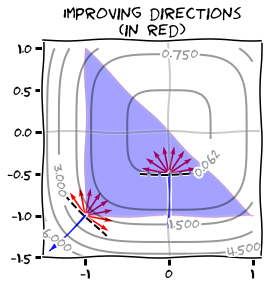
\includegraphics[width=0.5\linewidth]{images/improvingdirections.png} &
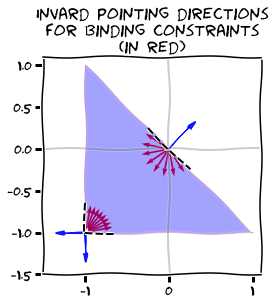
\includegraphics[width=0.5\linewidth]{images/inwarddirections.png} 
\end{tabular}
\caption{Cones for $(0,0)$, $(-1,-1)$ and $(0,-1/2)$.}
\label{figure:cones}
\end{figure}
\end{example}

\separator 

In the following sections we are going to discuss necessary and sufficient conditions for the existence of (strict) global minima for any consistent program $(P)$.  We are going to focus exclusively on the main results without showing their proofs (if interested in those proofs, consult \cite[lec6\_constr\_opt]{Freund2004nonlinear}).\index{Minimum!global}\index{Minimum!strict global}\index{Minimum!local}\index{Minimum!strict local}